\documentclass{article}

\usepackage[italian]{babel}     %testi autogenerati italiano
\usepackage{graphicx}           %per importare immagini
\usepackage{geometry}           %per gestire margini e spostamenti
\usepackage[raggedright]{titlesec}
\geometry {
    top=20mm,
    bmargin=20mm,
}
\usepackage{array}              %per colonne di width fissata
\usepackage{subcaption}         %tabelle divise
\usepackage{hyperref}           %links
\hypersetup{
    colorlinks=true,
    linkcolor=black,
    urlcolor=blue
}
%\usepackage[bottom]{footmisc}   %footnotes fissate a piè pagina
\usepackage{booktabs}           %per tabitem in tabular
\newcommand{\tabitem}{~~\llap{\textbullet}~~}
\renewcommand*{\thefootnote}{[\arabic{footnote}]}

\begin{document}

\setlength\parindent{0pt} %noindent automatico
\setlength\parskip{1em}

\begin{titlepage}
	\centering
	\hrule
	
	\vspace{6,5cm}
	{\Huge \textbf{Home Challenge \#4\\
		2020/21}\\}
		
		\vspace{0,5cm}
		\large {Prof. Cesana Matteo}
		
		\vspace{2,5cm}
		{
			\large
			\begin{tabular}{c c}
				Shalby Hazem Hesham Yousef & (Personal Code: 10596243) \\
			\end{tabular}
			
		}
		\vspace{4cm}
		
		\normalsize{17 May 2021}
		\vspace{0,2cm}
		
		\centering\hspace{0,2cm}
\includegraphics[scale=0.6]{./logo.png}
		\vspace{0,5cm}
		\hrule
		
		\end{titlepage}
		
		\pagebreak
		
		\pagebreak
		
		\section{Problem description} %1
		The mote  \texttt{\#1} sends requests (\textbf{REQ}) to the mote \texttt{\#2} every \texttt{1000 ms} (\texttt{1 Hz}) until the reception of an ACK message\footnote{after the reception of an ACK the mote   \texttt{\#1} stops.}.\\
        The mote  \texttt{\#2} replies to a mote  \texttt{\#1} request with a response (\textbf{RESP}) message containing the value from a “fake” sensor and the counter sent by mote \texttt{\#1}.
        
        \section{Results} %1
        Since the mote \texttt{\#2}, in the simulation, is booted with a five seconds delay compared to mote \texttt{\#1}, the first five REQ messages will not receive any ACK from Mote \texttt{\#2}.\\
        The only response sent from mote \texttt{\#2} is the consequence of the reception of the sixth REQ message (\texttt{counter=5}).\\ 
        The following image represents the simulated behavior.

        \begin{center}
        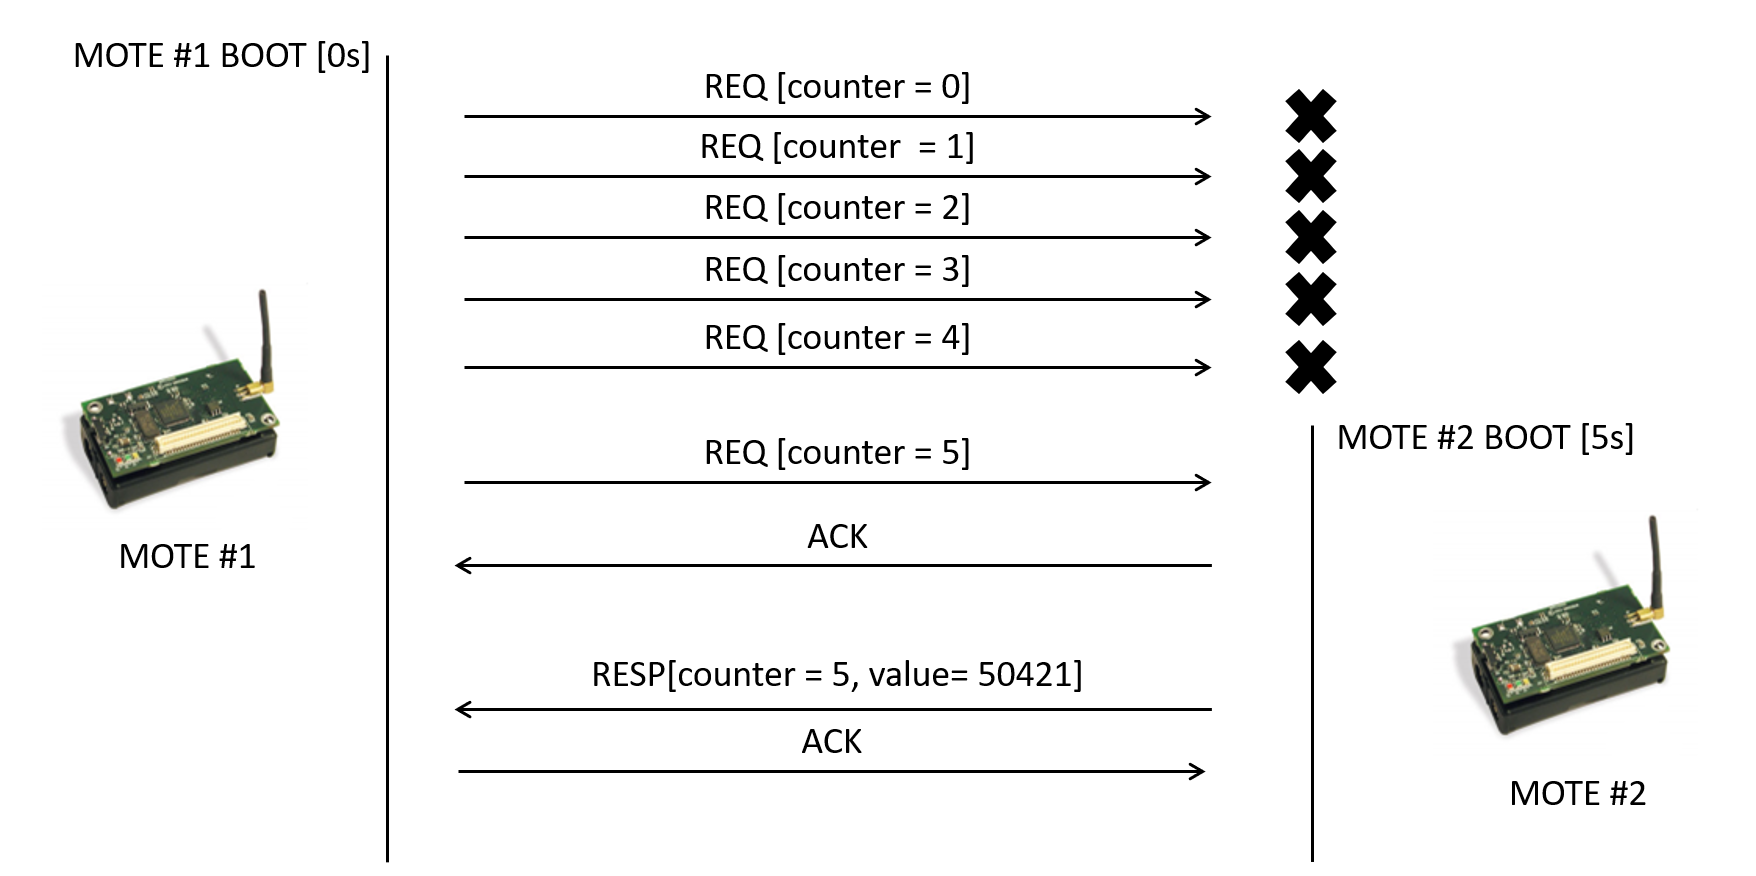
\includegraphics[width=1\textwidth]{./simulation.png}            
        \end{center}
        
        The previous image contains also an important result for the purpose of this homework, which is the value that mote \texttt{\#2} replay with to the request of mote \texttt{\#1}. The value we are talking about is \texttt{50421} and it is always the same in every simulation, due to the fact that we use a "fake" sensor, but in real world this value will change based on what the sensor captures.
        \\
        
        \pagebreak
		\pagebreak
		\clearpage
\end{document}